\documentclass[twoside,a4paper,11pt]{article}
\pagestyle{plain}
\pagenumbering{arabic}
\title{The Core Model and Sources of Data}
%\subtitle{Working Paper 001}
\author{Graeme Smith}
% \date{date text} just print the current date.
\usepackage[authoryear]{natbib}
\usepackage{amsmath}
\usepackage[left=2cm,top=3cm,right=2cm,bottom=3cm,bindingoffset=0.5cm]{geometry}
\usepackage{graphicx}
\usepackage{comment} 
\begin{document}

\maketitle
\begin{abstract} This note presents an outline of a Stock Flow Consistent (SFC) model to investigate the connection between global economic imbalances and global financial instability. The post-crisis financial literature reveals various views on the contribution of global imbalances to the financial crisis. A first group is concerned with the large current account imbalances that developed in the pre-crisis period especially in the US. Prominent in this group are the `global savings glut' view \cite{Bernanke2005},  the ‘excess demand for safe assets’ view \cite{Caballero2006} and the ‘Bretton Woods II’ view \cite{Dooley2003}. A second group gives more attention to the large international financial flows that built up in this period from which has emerged the `excess financial elasticity' view \cite{Borio2011b}. It is this view which underlies the model presented here.
\end{abstract}

The purpose of this note is to test the availability of economic and financial data to populate and calibrate an empirical model capturing the global financial flows in the pre-crisis period. Section 1 outlines the theory behind the model as set out by various authors in the financial literature following the crisis. Section 2 presents a first iteration of a model that would capture these flows. Section 3 lists publicly available data sources that could be used to populate the model.

\section{The Theory}
Among the suggested causes of the Global Financial Crisis, the extent of global macroeconomic imbalances ranks highly. Even in the pre-crisis period, economists and international agenies were drawing attention to these and especially to the yawning current account deficit of the United States. The analyses that were offered at the time could be roughly divided into three broad views of the phenomena, namely the `savings glut' view \cite{Bernanke2005},  the `excess demand for safe assets view' \cite{Caballero2006} and the `Bretton Woods II' view \cite{Dooley2003}. These three views have in common that they focus on current account imbalances and the net financial flows that they induce, but also they share the view that the mechanism by which these imbalances led to financial instability is through downward pressure on US interest rates which stimulated the housing bubble. This mechanism is essentially a restatement of the `loanable funds' theory which holds that credit supply is limited by current saving. \cite{Lindner2015} uses a simple stock flow consistent model to show that credit supply and saving are quite distinct phenomena which undermines the basis for these three views.

In contrast to these three views, a number of authors (e.g.  \cite{Borio2011d}, Golub1990, Obstfeld2012a) have contended that it is the \emph{gross} financial flows that are important, and that a preoccupation with the current account diverts attention away from this. In \cite{Borio2015a} the distinction between net and gross financial flows is explained by the distinction between saving and financing. ``Saving, a national accounts concept, is simply income (output) not consumed; financing, a cash flow concept, is access to purchasing power in the form of an accepted settlement medium (money) ... investment, and expenditures more generally, require financing, not saving. And financing is a gross, not a net, concept'' \cite[p1-2]{Borio2015a}. ``This distinction is precisely what is lost in the prevailing analytical frameworks, which have tended to treat money and finance as veils of little or no consequence'' (p.2). This suggests that the failure to distinguish saving and financing could be attributable to the preoocupation in mainstream macroeconomics with \emph{real} resource flows as opposed to monetary flows arising from the principle of the neutrality of money.
 
These considerations have led to the `excess financial elasticity' view \cite{Borio2011d} which shifts attention  from current account balances to the gross financing flows that are generated by international economic activity, including portfolio and speculative flows. It argues that the growing capital flows (mainly into the US) in the pre-crisis period led to domestic credit expansion and asset price inflation, leading to inflated balance sheets  -- this is the excess financial elasticity that they refer to. It means that the international monetary and financial system (IMFS) was unable to absorb and safely recycle the elevated level of financial flows. They focus on the monetary regimes that set monetary conditions in the various currencies, the financial regimes that set constraints on financial intermediation in the various national jurisdictions, and on the interaction between the two.

This interaction between international capital flows and domestic credit growth is further investigated in \cite{Lane2014a} with an econometric study using data from 1993-2008 and establish a clear relation between debt inflows and domestic credit growth. \cite{Avdjiev2015} present a typology of international flows. As well as pure inflows and outflows such as would be required to finance current account deficits, there are also `pure offshore' transactions and `round-trip transactions'. The latter are described in detail in \cite{Acharya2010} which documents the practice of European banks setting up off balance sheet investment vehicles that were funded by short-term borrowing from US money market mutual funds and invested in longer term US securities, mainly mortgage backed securities. This is an example where the net flows would have been zero, but the gross flows enormous since the short-term funding was 30 days or less so the entire portfolio would have been rolled over in every period.

\cite{Bertaut2012} also argue that the global savings glut view is incomplete as an explanation of global  financial  imbalances in this period. Because the GSG (Global Savings Glut) countries (by which they mean the Asian countries following an export-driven growth model) for the most part restricted their U.S. purchases to Treasuries and Agency debt, their provision of savings to the risky subprime mortgage borrowers was indirect, pushing down yields on safe assets, and driving a `search for yield' on the part of other investors increasing their appetite for alternative investments. A more complete picture of how capital flows contributed to the crisis must pay attention to the large inflows from European countries, most of which went into asset-backed securities (ABS), including mortgage-backed securities and other structured investment products rather than `safe assets' (treasuries and agency debt). The current account position of these European countries was roughly in balance overall, with some running a significant surplus (Germany, Netherlands) and others with significant deficits (UK). Hence the current account position was not a crucial factor in understanding the global imbalances.

Further support for this view comes from \cite{Acharya2010} by analyzing the geography of `financial conduits' set up by large commercial banks. They show that  banks located in both surplus countries and deficit countries manufactured `riskless assets' by selling short-term asset-backed commercial paper to risk-averse investors, predominantly US money market funds, and investing the proceeds primarily in long term US assets (mainly ABS). Many of these conduits were sponsored by European banks while the short-term funding (usually 30 days or less) was coming from the US. When the credit quality of these securities became known in 2007, the `conduits'  were unable to roll over the short-term funding and the sponsoring banks had to provide a liquidity backstop  \cite{Baba2009} which led to a global `dollar shortage' once the crisis began \cite{McGuire2009}. \cite{Brender2010} discuss international `risk taking chains' that recycled some of the GSG funds into riskier US investments. This model will capture these international flows and their impact on the financial instability of the US economy.

\subsection{Financial Instability}
The effect of these financial flows was to undermine financial stability in the affected economies. The US financial system was required to `recycle' financial flows of approximately 20 percent of GDP at the peak in 2007. The `excess financial elasticity' view asserts that even the very advanced US financial sector was unable to handle such flows without leading to excessive credit expansion and consequent financial instability.

The dynamics of the financial instability generated by excessive financial flows has been described by many authors, the following from \cite{Obstfeld2012a} captures the concepts very succinctly, ``In credit booms, asset values rise, improving balance sheets and facilitating the further expansion of credit. As a result, subsequent collapses are all the more traumatic. (The carry trade involves similar dynamics.) A capital inflow episode likewise may strengthen financial sector assets and even the NIIP in the receiving country in a way that pushes domestic borrowing beyond the point of true sustainability. This often sets the stage for a disorderly collapse later on. In diagnosing such situations, it is essential to keep the underlying credit flows in clear view'' \cite[:p479]{Obstfeld2012a}.

\cite{Miess2015} describe this effect as  'Kindleberger cycles' and combine this with a stock flow consistent model in which the positive feedback effects of expansion of credit may be directed not at productive investment but at acquisition of existing assets leading to increases in asset prices and hence to their collateral value. This raises the creditworthiness of agents which encourages a further round of credit expansion, the process continues in a self-perpetuating spiral. The spiral can be ended by any one of a number of triggers -- a reluctance of creditors to continue to provide credit, an unexpected fall in asset prices, rising defaults by overleveraged debtors and others.

The most developed model of financial instability is Minsky's `Financial Instability Hypothesis' \cite{Minsky1986}. The model has been successfully coupled to stock flow consistent models to capture the dynamics of credit creation and financial instability by a number of authors, \cite{Caverzasi2015b}, \cite{Bezemer2011}, \cite{DosSantos2004}, \cite{Dafermos2015a}  provide a small sample.

The core model builds on these examples to explain the effect of excess financial elasticity on financial stability in terms of a Minsky cycle. 

\section{The Model}
Technically, an SFC model is formulated as a dynamic system of difference equations.
The behaviour of the system depends on the functional relations between the
variables (i.e. the model equations), the parameter values, and the initial conditions. A
model can either be unstable with the value of the variables in time going to infinity
(diverging behavior), or converge to a stationary state or a limit cycle (converging behaviour). There may also be the possibility of chaotic behaviour. A particular case of divergent behavior has been termed a `steady state' \cite[:p9]{Caverzasi2014a} where stocks and flows are growing at a constant rate.

They also distinguish between \emph{fully empirical models} and \emph{empirical models} (unfortunate nomenclature) in the following way: in fully empirical models, all the parameters are estimated not calibrated (see later for explanation of the diffference) and the models are used to predict variations in endogenous variables based on different scenarios, starting from the present state of economy. By contrast, empirical models extract stylised facts from empirical data and then conduct simulations on the basis of these facts. The simulations start from a steady state that is not necessarily connected to the present situation. There are two styles of fully empirical models -- the Levy style, and the Limerick style \cite{Kinsella2012b}. The Levy style assumes fixed parameters estimated using econometrics whereas the Limerick model estimates fixed parameters only when necessary (if there is more than one parameter per independent equation) and calibrates the others. They define estimation as follows: a parameter is assumed constant over a time span and estimated using econometric methods such as ordinary least squares, maximum likelihood, etc. Calibration is the process of finding a value for each parameter, in each period, such that the model replicates the dataset. In that sense, calibration has no predictive power since it does not give any insight on parameters’ future values. However, filtering techniques can be used on these calibrated parameters in order to obtain a trend and thus predict future values. Most models are calibrated to a stationary state, which is used as a basis for policy experiments or the analysis of shocks.  The calibration procedure fixes values of the equation parameters  to ensure that model variables will fit the observed data.

An alternative for fully empirical models is to analyse dynamic behaviour in terms of stock-flow norms \cite{Godley1999b}. In \cite[p42]{Godley1983} the authors assert that ''stock variables will not change indefinitely as ratios to related flow variables'' and this principle provides a basis for analysis of system dynamics and stability. Rather than evaluating parameters in behavioural equations to support analysis, key stock-flow norms provide the means for understanding relationships between variables of the model.  The core model described here will follow this approach in the context of a fully empirical model.

The model will be centred on the US economy with  three foreign blocs -- China, which will act as a proxy for the global savings glut (GSG) countries, Europe (the eurozone + UK) which will capture the investment-driven finanial flows and the rest of the world (ROW) which will be a residual to preserve the adding up constraints. The model will use changes in national balance sheets to capture the effects of international financial flows on the financial stability of the individual economies. Figure \ref{fig:bs} shows the balance sheet of the model. At the highest level there are two sectors, the US and the rest of the world (ROW) which are further decomposed into a domestic non financial sector whiich comprises households, firms and the government; the ROW is made up of China as a proxy for the GSG countries and the UK and eurozone as sources of the financial inflows. Not all sectors of the ROW sectors are used since the focus is on financial flows to the US. 

\begin{comment}
The assets are 
\begin{itemize}
\item[] Real Assets, which includes household real estate
\item[] Deposits
\item[] Equities
\item[] Bank Loans, including household mortgages
\item[] Treasuries and Agencies, these are the main classes of government debt. 
\item[] Money Market Mutual Funds (MMMF)
\item[] Securities, asset-backed securities and corporate bonds
\item[] CB advances
\item[] Reserves
\end{itemize}
\end{comment}

\begin{figure}
  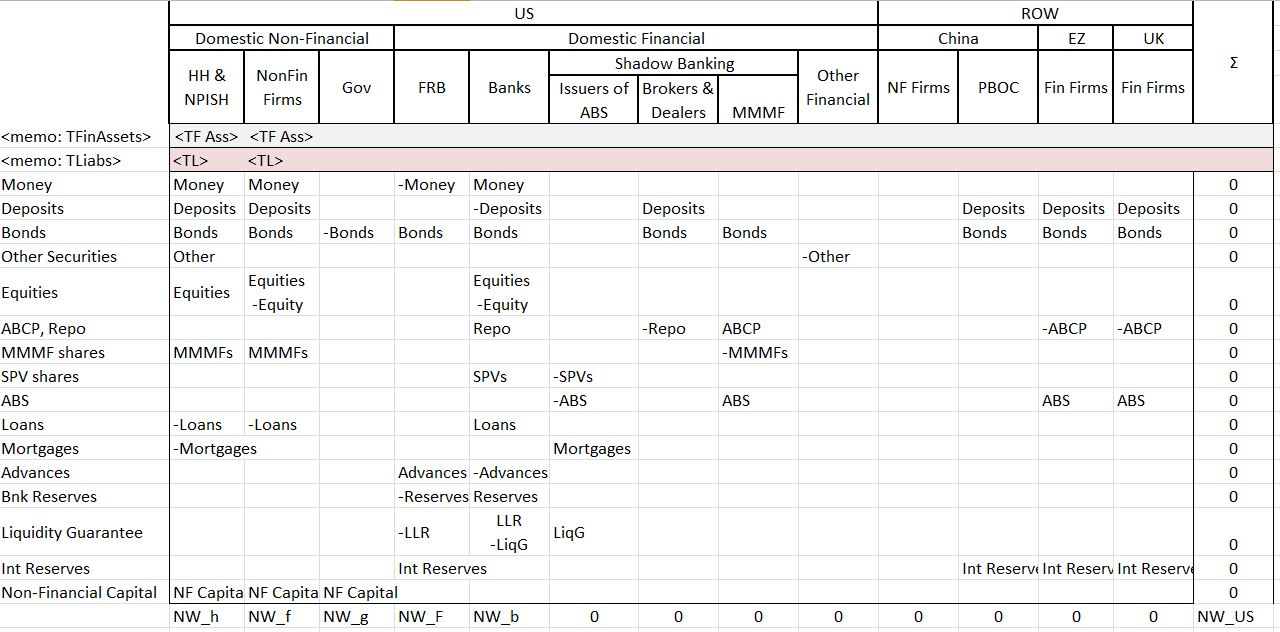
\includegraphics[width=\linewidth]{balance-sheet.jpg}
  \caption{Balance Sheet for Core Model}
  \label{fig:bs}
\end{figure}

\begin{comment}
%\begin{table}[h]
\begin{center}
\begin{tabular}{llllllll}
\hline
& HH & NFF & B & OFI & G & CB & $\Sigma$  \\
\hline
Real Assets &  &  &  &  &  &  & 0 \\
Deposits &  &  &  &  &  &  & 0 \\
Equities  &  &  &  &  &  &  & 0 \\
Bank Loans &  &  &  &  &  &  & 0 \\
T Bills  &  &  &  &  &  &  & 0 \\
MMMF &  &  &  &  &  &  & 0 \\
Securities  &  &  &  &  &  &  & 0 \\
CB advances  &  &  &  &  &  &  & 0 \\
Reserves  &  &  &  &  &  &  & 0 \\
Net Worth  &  &  &  &  &  &  & 0 \\
\hline
\end{tabular}
\end{center}
\caption{The Balance Sheet for a typical trading bloc}
\end{table}
\end{comment}

Figure \ref{fig:hh} shows  the dynamics of the balance sheet of the household sector over the period 2000Q1 to 2015Q2. The data are taken from the Federal Reserve Board's Z.1 flow of funds accounts. It shows the decline in household net worth in the post-crisis period and the associated loss in value of non-financial assets.

\begin{figure}
  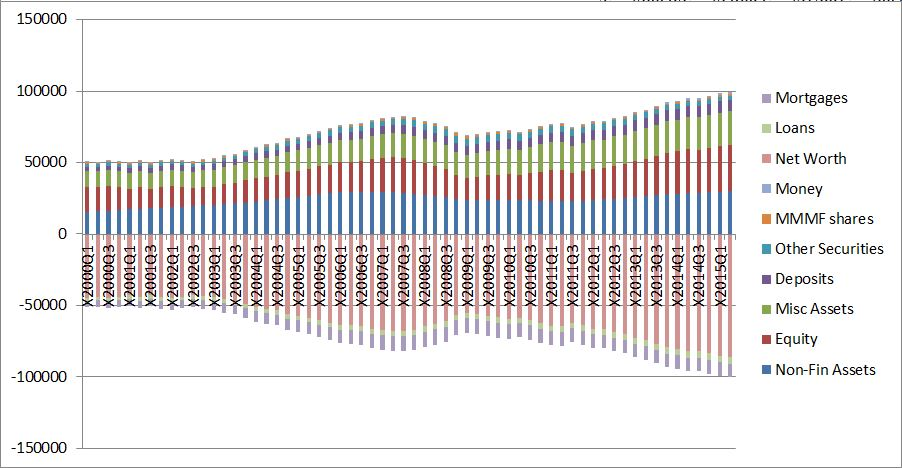
\includegraphics[width=\linewidth]{hh.jpg}
  \caption{Dynamics of the Household sector, 2000-2015. \emph{Source FRB Z.1} }
  \label{fig:hh}
\end{figure}

The corresponding transaction matrix is shown in figure \ref{fig:tx}. The starting point for the analysis of transaction flows in this model is in line 3 -- net lending and borrowing -- which is derived from both the balance of payments accounts and the NIPA accounts. In theory, the rest of the world’s net lending or net borrowing in the capital account should equal that of the total domestic economy. In practice, however, the difference between these two measures is equal to the discrepancy between the income and product sides of the NIPAs. In figure 2 the flows are shown as changes in the stock values of the assets from the balance sheet in figure \ref{fig:bs}.  In the financial account of the Balance of Payments, each flow is assigned to a category from the financial accounts of the balance of payments:
\begin{itemize}
\item[] FDI
\item[] Portfolio Investments
\item[] Derivatives
\item[] Other Investments
\item[] Reserves 
\end{itemize}

In the financial account of the National Income and Product accounts, each flow accumulates to either of `Net Acquisition of Financial Assets' (NAFA) or `Net Incurrence of Liabilities' (NIL) for each sector. The format of figure \ref{fig:tx} attempts to make all of these linkages explicit. Figure \ref{fig:nlb} shows a sectoral breakdown of NLB as the difference between NAFA and NIL for the US.

\begin{figure}
  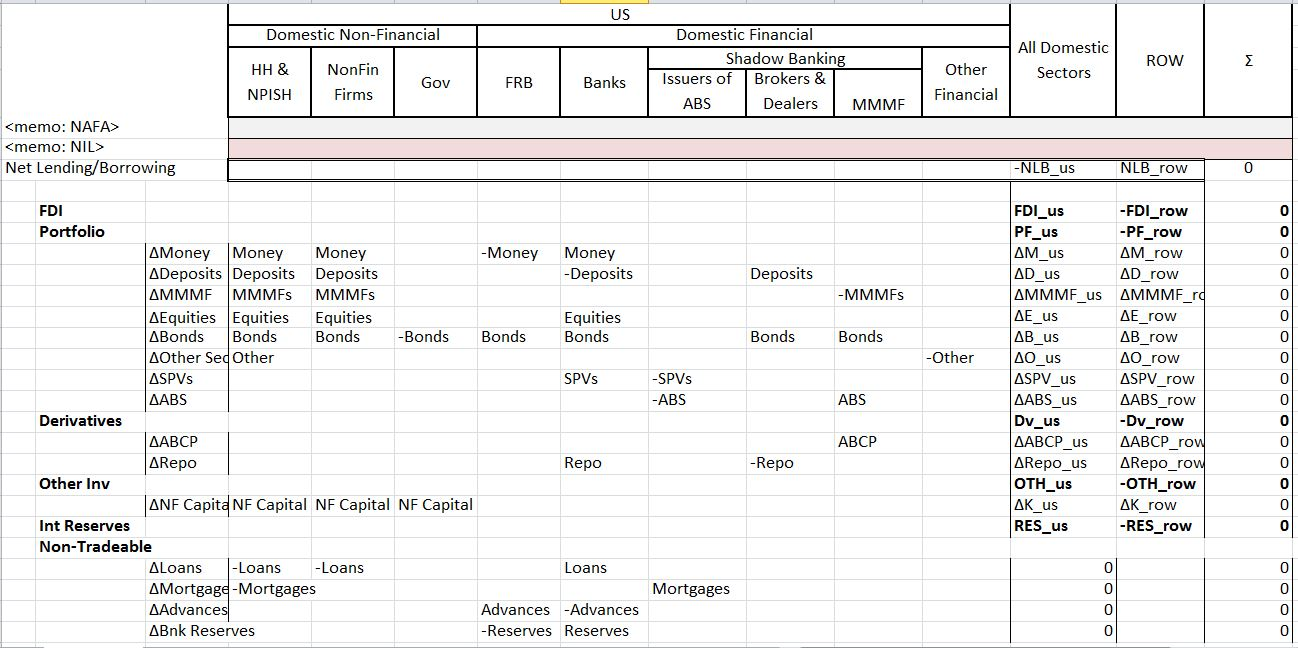
\includegraphics[width=\linewidth]{trans-matrix.jpg}
  \caption{Transactions Matrix for Core Model}
  \label{fig:tx}
\end{figure}

\begin{figure}
  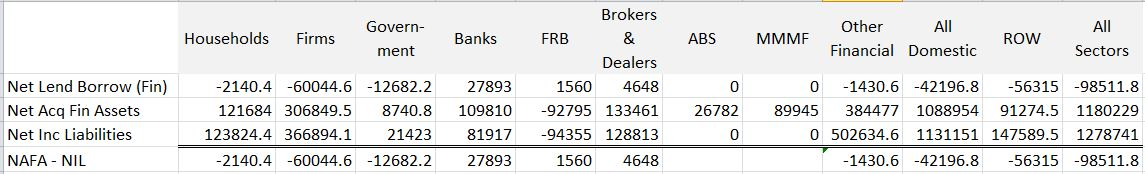
\includegraphics[width=\linewidth]{NLB.jpg}
  \caption{Sectoral breakdown of NLB}
  \label{fig:nlb}
\end{figure}

%\pagebreak
\section{The Data Sources}
One of the reasons for centering the model on the USA is the ready availability of US data, notably  from the US Flow of Funds maintained by the Federal Reserve Boards.   
\subsection{The United States}
The Federal Reserve Board's statistical release Z.1 is  usually referred to as the `Flow of Funds accounts (FoF) or the ``Financial Accounts of the United States'' to give it its full name. It consists of the Flow of Funds, Balance Sheets, and Integrated Macroeconomic Accounts. The flows in these accounts are normally expressed as net flows. To separate them out into gross flows, the Treasury International Capital (TIC) system provides detailed data on the composition of U.S. capital flows and the U.S. external position by country and instrument. In addition, the Bank of International Settlements (BIS) data on international banking positions, and the IMF’s Coordinated Portfolio Investment Survey (CPIS), provides geographic breakdowns of many countries’ external securities claims.

The FoF provides the following information:
\begin{itemize}
\item[] Matrices summarizing stocks and flows across sectors, tables on debt growth, net national wealth, gross domestic product (GDP), national income, saving, and so on
\item[] Flows of financial assets and liabilities, by sector and by financial instrument
\item[] Stocks of financial assets and liabilities, by sector and by financial instrument
\item[] Balance sheets, including nonfinancial assets, and changes in net worth for households and nonprofit organizations, nonfinancial corporate businesses, and nonfinancial noncorporate businesses
\item[] The Integrated Macroeconomic Accounts (IMA). These relate production, income, saving, and capital formation from the national income and product accounts (NIPA) to changes in net worth from the “Financial Accounts” on a sector-by-sector basis. The IMA  are based on international guidelines and terminology defined in the System of National Accounts (SNA2008).
\end{itemize}
The sectors include:
\begin{itemize}
\item[] Households and Nonprofit Institutions Serving Households (NPISH)
\item[] Nonfinancial Noncorporate Businesses
\item[] Nonfinancial Corporate Businesses
\item[] Financial Businesses
\item[] Federal Government
\item[] State and Local Governments
\item[] Rest of the World
\end{itemize}
For the purposes of this study the two non-financial sectors will be merged to give the NFF sector, state and local governments will be merged with the federal government to give sector G and data for China and the EU will be disaggregated from the Rest of the World sector. There are further detailed tables that further disaggregate certain sectors, e.g. the monetary authority is separated out in tables F.109 and L.109 from which the sector CB can be formed. Other detailed tables give a breakdown of the Financial sector from which the MMMF sector can be formed. 

%Particularly important tables will be:
%\begin{itemize}
%\item[] D.1 Debt Growth by Sector
%\item[] B.1 Derivation of U.S. Net Wealth
%\item[] F.4 Saving and Investment by Sector
%\item[] F.6 Derivation of Measures of Personal Saving
%\item[] L.6 Assets and Liabilities of the Personal Sector
%\item[] 
%\item[] 
%\end{itemize}

\subsection{The EU}
\subsubsection{The Eurozone}
Eurostat accounts: national income accounts and balance of payments for all EU countries.

ECB data:
The Statistical Data Warehouse (http://sdw.ecb.europa.eu/reports.do). This includes the economics bullsting and the statistics bulletin which consists of the following sections:\\
\begin{quote}
Euro area overview S 5\\
1 Monetary policy statistics S 6\\
2 Money, banking and other financial corporations S 10\\
3 Euro area accounts S 26\\
4 Financial markets S 34\\
5 Prices, output, demand and labour markets S 46\\
6 Government finance S 55\\
7 External transactions and positions S 60\\
8 Exchange rates S 72\\
9 Developments outside the euro area S 74\\
Notes S 76\\
\end{quote}
Section 7 provides portfolio flows and investments in financial derivatives.

\subsubsection{UK}
UK National Income Accounts:\\
The Pink Book:\\
The Blue Book:

\subsection{China}
TBD

\subsection{Data Disaggregation}
The flows in these accounts are normally net flows. To split them out into gross flows additional, more-detailed data will be required. These sources include: 1) additional breakdowns that are provided in the US Flow of Funds accounts, as well as the euro area and U.K. Balance of Payments data; 2) BIS locational data, in which the Bank of International Settlements splits banks’ cross-border positions into those with other banks and those with non-banks; and 3) aggregate balance sheet data published by the euro area and the U.K. for banks, other financial firms, and non-financial firms.

%\subsection{Bank of International Settlements (BIS)}

\bibliographystyle{plainnat}
\bibliography{WN002}
\end{document}
